%! TeX root = ../charles/en/thesis.tex

\chapter{Background}
\label{chap:bg}

In this chapter, we briefly cover progress in obtaining useful representations
of language (Section \ref{sec:lm}), images (Section \ref{sec:imrec}), and
efforts to combine these two modalities (Section \ref{sec:vlm}). We then
look at the extension of vision and language models to videos (Section
\ref{sec:vidlm}), which introduces the extra complexity of reasoning across
sequences of images, and optionally adding a further modality, audio. Finally,
we explore the literature on temporal reasoning in language and in vision
(Section \ref{sec:tempreason}).
%We finish the chapter with an introduction to and motivation for studying the
%task of video question answering (Section \ref{sec:vidqa}).

\section{Language Modeling}
\label{sec:lm}

Language modeling is the task of predicting the next word given some number of
previous words. A neural language model~\citep{bengio2003nlm} performs this by
receiving as input to a feedforward neural network a representation of previous
words in a sequence and outputting a probability distribution over possible
words. The probability of a sequence of $T$ words $w_1^T$ is thus the
combined probability of all words given their context:
$$\hat{P}(w_1^T)=\prod_{t=1}^{T}\hat{P}(w_t|w_1^{t-1})$$
The conditional probability can be approximated by using a fixed context
length, $N$, $$\hat{P}(w_t|w_1^{t-1})\approx\hat{P}(w_t|w_{t-N+1}^{t-1})$$,
greatly reducing the computational requirements for longer sequences.

\subsection{Recurrent Neural Networks}
\label{ssec:rnn}

The recurrent neural network (RNN) takes individual items from a sequence, one
at a time, and outputs a prediction based on the single unit and a hidden
state.  The hidden state is a recursive unit learnt from previous hidden
states, so that at timestep $t$, the hidden state $h_t$ is a combination of the
previous hidden state $h_{t-1}$ and the current input $x_t$. The hidden state
is therefore a representation of the entire input sequence up to time $t$. This
avoids the problem faced by feedforward neural language models of only
representing a limited context window of size $N$. In theory, an RNN can
represent an unlimited context.

In practice, RNNs struggle to encode long-distance dependencies well, with the
information encoded in hidden states being biased towards more recent items of
the input, and struggling from the vanishing gradient problem, whereby repeated
matrix multiplications for backpropagation through time drive the gradient to
zero. The main extension to the RNN, the long short-term memory (LSTM)
network~\citep{hochreiter1997lstm}, modifies the architecture of the recurrent
unit to include three gates: the forget gate, the add gate, and the output
gate. Combined, these three gates keep the context vector, the previous hidden
state, simple by removing information considered no longer useful, add useful
information from the current input, and output information considered useful
for the current hidden state.

RNNs are often used in sequence-to-sequence, or encoder-decoder, set-ups, in
which the input sequence is processed by the encoder section, creating a
context vector which is a representation of the entire input sequence. This is
then fed as the initial hidden state of a decoder network to generate the
output. The benefit of this is that the output size is not related to the input
size. For tasks such as machine translation, image captioning, or open-ended
question answering, the ability to generate an answer is critical.

The bottleneck problem is alleviated slightly by the attention
mechanism~\citep{bahdanau2015attention}, where an additional context vector is
used by the decoder to dynamically attend to different hidden states of the
encoder based on the current input token in the decoder. This context vector is
created by a weighted sum of encoder hidden states, recomputed at each timestep
during decoding. Attention with RNNs improved the state of the art in machine
translation, particularly on sentences with longer input. It has also been used
in vision and language models to attend to key parts of the image vector
for visual question answering~\citep{yang2016san}.


\subsection{Transformer}
\label{ssec:transformer}

\citet{vaswani2017attention} introduced the Transformer architecture for
sequence tasks, replacing the recurrent nature of the RNN and its variants with
multi-head self-attention. This allows for parallel computation since
computation at each timestep is independent of all others, greatly increasing
the ability to train on larger and larger data and model sizes. Self-attention
assigns attention scores to each item of the input sequence itself, regardless
of input size, to compute a representation of the sequence. The Transformer
uses stacked layers of self-attention to capture the many ways that an input
sequence can relate to itself. Each self-attention head can learn to encode
different relationships between sequence tokens, and these heads are combined
and linearly projected into the original dimensionality.
\citet{vaswani2017attention} use attention between the encoder and decoder, so
each position in the decoder can attend to all items of the input sequence, and
further use self-attention in both the encoder and decoder. In the decoder, a
modification is made to prevent knowledge of future information being
generated, masking out all values in the input that correspond to future input
connections. Finally, positional encodings are included for each token to keep
some notion of sequence order that would otherwise be lost from the RNN
architecture. The Transformer achieved state of the art performance on machine
translation, and has since been used as the de facto architecture for many
sequence tasks, in both language and vision.

\subsection{Masked Language Modeling}
\label{ssec:mlm}

BERT~\cite{devlin2019bert} uses only the encoder layers of the Transformer to
create strong representations of an input sequence. Since it is trivial to
predict the next token in a sequence when provided with the entire context,
BERT, and its descendants such as RoBERTa~\citep{liu2020roberta}, train on a
masked language modeling objective on unlabeled data, where the task is to mask
some percentage of the input tokens at random, and then predict those masked
tokens.

These representations on their own are not especially useful, but once trained,
they provide a great starting point for finetuning to a specific task, where
there may not otherwise be enough data to learn these rich representations of
language. Downstream tasks can include question answering, natural language
inference, or sentence classification. Pre-training then finetuning has become
a common paradigm due to the relative low cost of finetuning once a large model
has been pre-trained. BERT achieved state of the art on eleven NLP tasks, all
of which were finetuned in less than an hour on a TPU. BERT has successfully
been adapted to vision and language models, as we will discuss in
Section~\ref{sec:vlm}.


\section{Image Recognition}
\label{sec:imrec}

A key part of video and language models is learning representations of frames
in sequence, which involves the classical tasks of object detection, image
segmentation, and image classification. Much like in NLP, the standard approach
is to pre-train on large image datasets and finetune to a specific desired
task. Convolutional neural
networks~\citep{lecun1989lenet,krizhevsky2012alexnet,he2016resnet} use
convolution kernels, pooling, and optionally normalisation, dense or residual
layers to create representations of image features.
AlexNet~\citep{krizhevsky2012alexnet} uses a multi-layer convolutional neural
network (CNN) to classify images from ImageNet~\cite{imagenet}, a dataset of
over 15 million images from around 22,000 categories, and was the first to show
the scaling power of large datasets and model sizes for producing strong image
features. 

There have been attempts to combine CNN architectures with self-attention
mechanisms. This may provide more scope for non-local computation which may be
required on tasks such as object detection with large objects. However, due to
the quadratic cost of self-attention in the number of pixels, naive
implementations are infeasible, and approximations struggle to scale
efficiently~\cite{carion2020detr}. The Vision Transformer~\cite{dosovitskiy2021vit}
does away with the CNN for image recognition, and uses an adapted version of
the Transformer for greater scalability.


\subsection{Vision Transformer}
\label{ssec:vit}

\cite{dosovitskiy2021vit} introduced the Vision Transformer (ViT), which takes
the impressive performance of the Transformer architecture on sequence tasks
and applies it to image tasks. The authors represent an image as a sequence of
patches of an image, with an extra patch embedding added alongside the
positional embedding of the Transformer \cite{vaswani2017attention} to maintain
the 2-dimensional information of an image when projected into a linear
sequence. The model is shown in Fig.~\ref{fig:vit}.  The Vision Transformer
matched or exceeded state of the art on many image classification datasets,
while being trained for comparatively less time.

\begin{figure}[htpb]
	\centering
	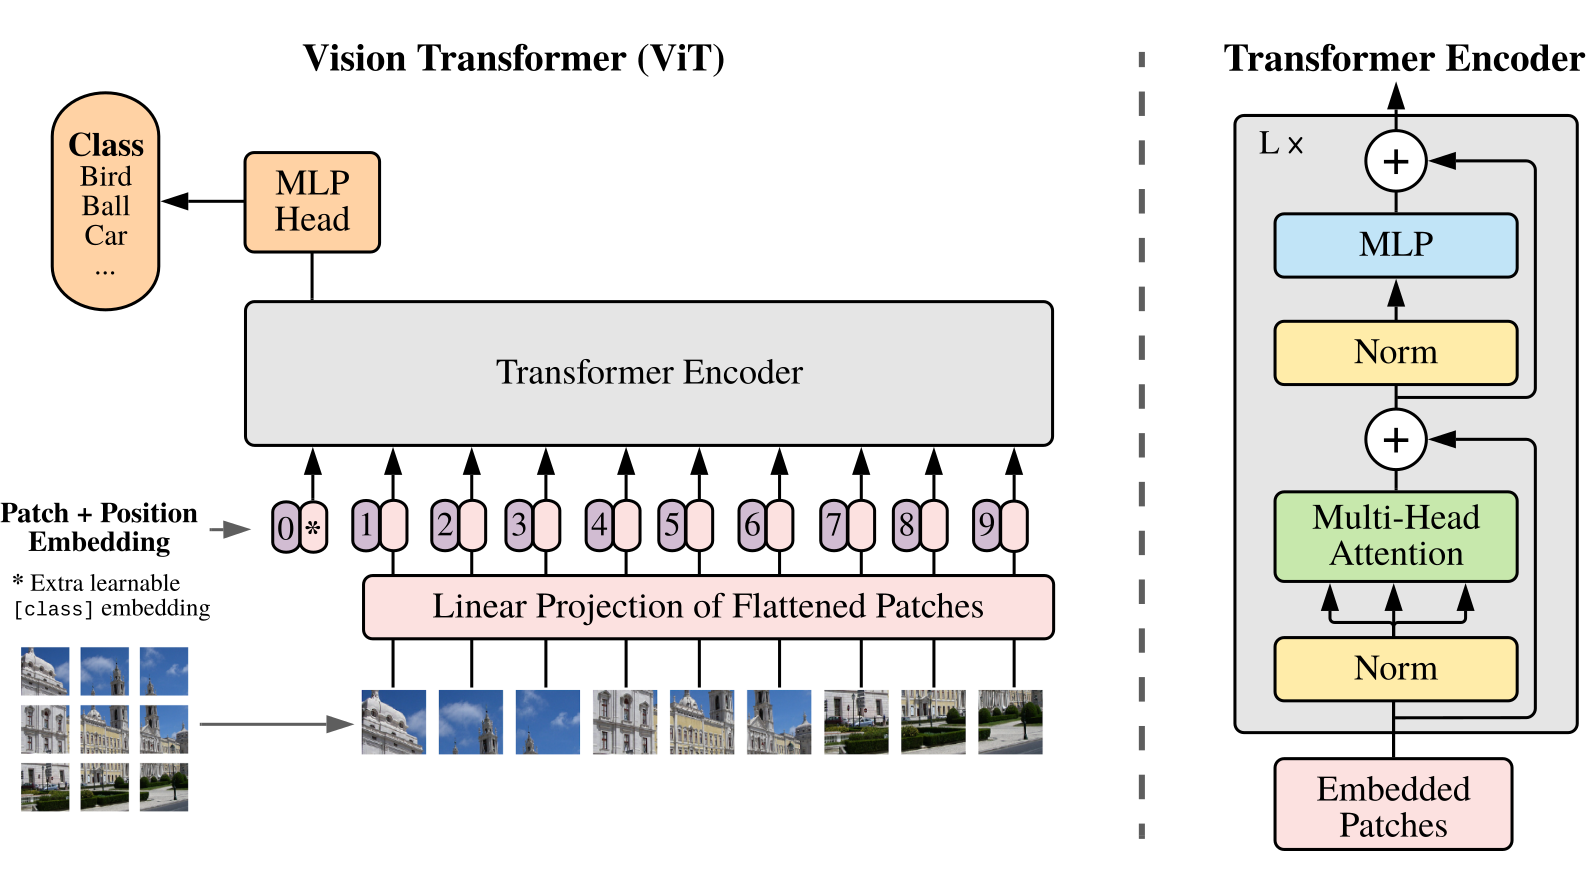
\includegraphics[width=0.8\textwidth]{vit.png}
	\caption{The Vision Transformer splits an image into patches, embeds them,
		and feeds them into a Transformer encoder. Classification is learned
		via an MLP head following the encoder. Figure reproduced
		from~\cite{dosovitskiy2021vit}}
	\label{fig:vit}
\end{figure}


\subsection{CLIP}
\label{ssec:clip}

\cite{radford2021clip} introduced CLIP (Contrastive Language-Image
Pre-training), which uses the Info-NCE loss~\citep{oord2019infonce} to jointly
learn relationships between encodings of text captions and extracted feature
representations of associated images. The Info-NCE loss trains a multimodal
embedding space to maximise the cosine similarity of matching pairs of captions
and images, while minimising the cosine similarity of non-matching pairs in the
batch. The approach is shown in Fig.~\ref{fig:clip}. A key part of this
approach is using a very large batch, so that there are many incorrect pairings
to learn from. \cite{radford2021clip} use a batch size of 32768. The text
encoder is a Transformer~\citep{vaswani2017attention}, and their best model
uses a Vision Transformer~\citep{dosovitskiy2021vit} as the image encoder.

\begin{figure}[htpb]
	\centering
	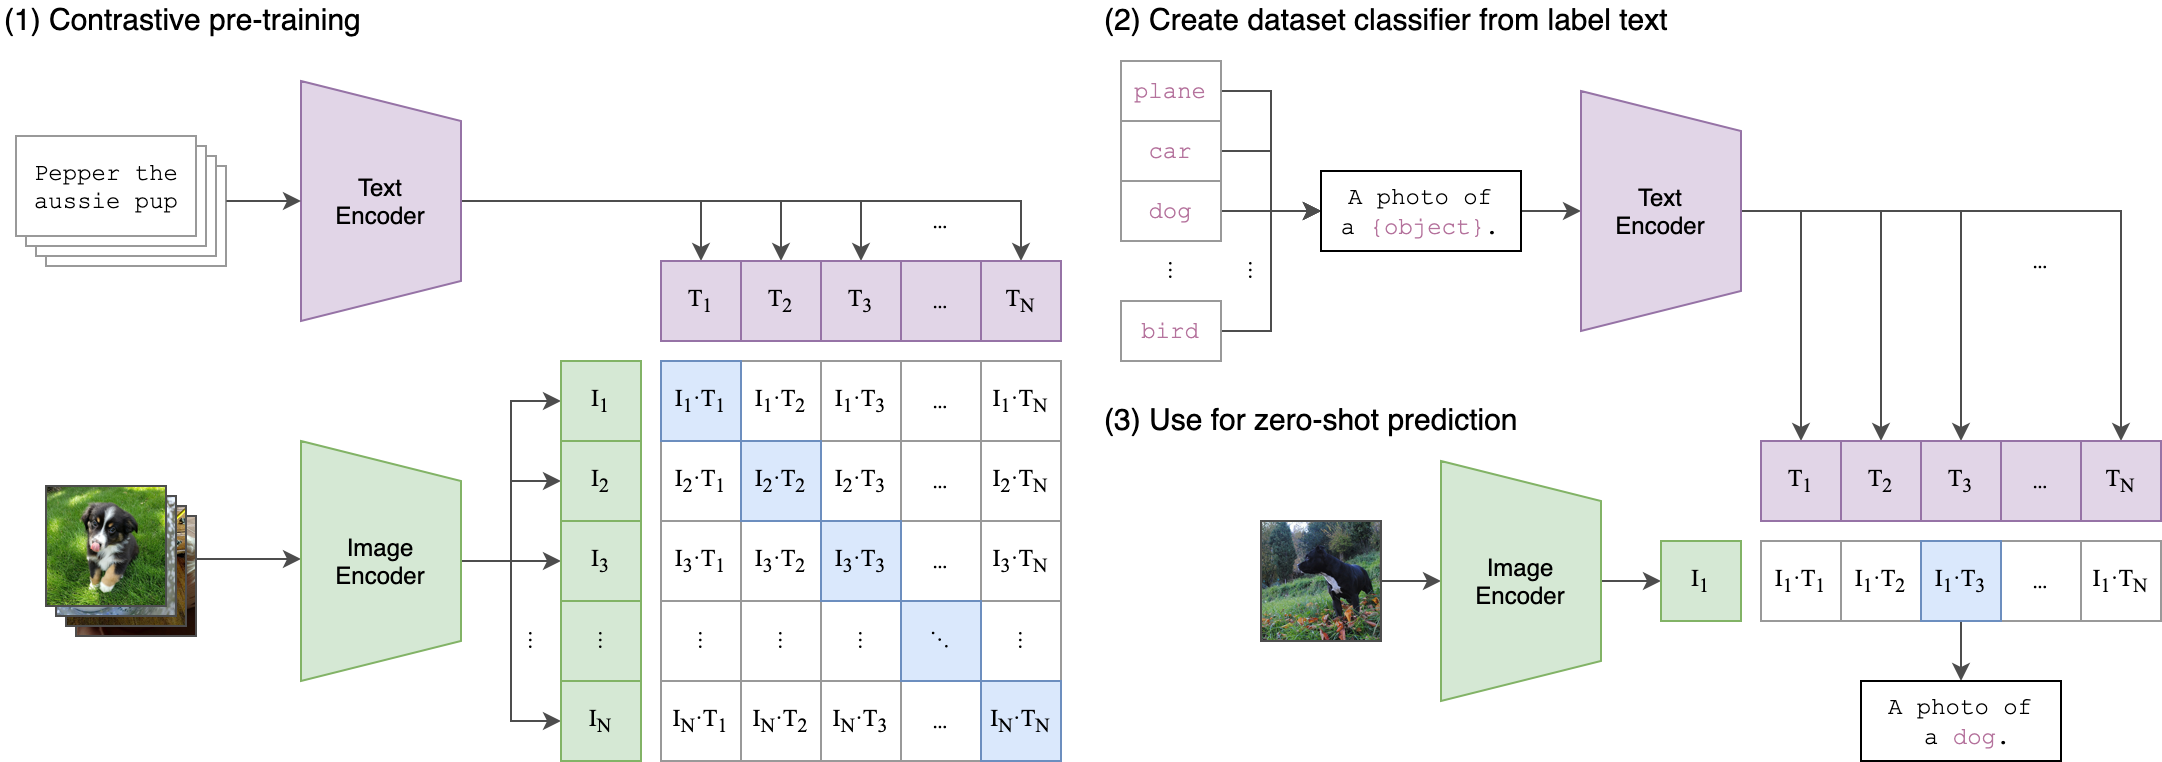
\includegraphics[width=\textwidth]{CLIP.png}
	\caption{CLIP. From~\cite{radford2021clip}}
	\label{fig:clip}
\end{figure}

The model enables zero-shot transfer to many downstream computer vision
classification tasks by predicting the most probable (image, text) pair when
given an image and a set of text prompts with each class embedded in the prompt
achieving performance comparable to or surpassing the previous state of the art
by finetuned models. The representations learned by the contrastive
pre-training objective have wide applicability to a range of VLM and Video
Language Models, particularly as frozen features from which to add smaller
modules on top for adapting to vision and language
tasks~\citep{alayrac2022flamingo,lin2022evl,lei2021clipbert}. We discuss some
of these models in Section~\ref{sec:vidlm}, and consider the limitations and
possible expansions of the contrastive pre-training method
in Section~\ref{sec:contrastive}.


\section{Vision and Language Models}
\label{sec:vlm}

One criticism of language models is that the representations learned by
training a model to predict the next word fail to learn any kind of
meaning~\citep{bender2020climbing} without reference to the real world. Models
trained in this way learn connections between surface forms, but no grounded
meaning between the form and intent portrayed through the form. A way to create
grounded representations may be to combine the two modalities of language and
vision through multimodal embeddings. A key challenge in recent years has been
to find suitable methods for creating these shared representations.

Following the strong performance in NLP of BERT~\citep{devlin2019bert},
\cite{li2019visualbert} extend BERT to include visual features extracted from a
CNN as well as text tokens as input to a Transformer encoder, implicitly
discovering a joint representation between the two modalities. The authors use
the self-attention mechanism to align elements of the input text and regions in
the input image, and pre-train on two visually-grounded language model
objectives. The authors finetune and evaluate on a range of vision and language
applications, including visual question answering (see below).

%\cite{lu2019vilbert}

Other approaches take frozen encodings of image, text, or both, and learn a
shared embedding space on top of this (e.g. BLIP-2 \cite{li2023blip2})

%Many approaches, joint training with concatenated image and text features into
%BERT (VisualBERT), learning both image and text features concurrently.


\subsection{Visual Question Answering}
\label{ssec:vqa}

Visual question answering is the task of answering questions given text and an
image. There are a wide range of datasets (name some). A challenge in creating
datasets is to ensure that there are few statistical biases or shortcuts in the
answer distribution that a model can exploit without a true understanding of
the scene. For example, models trained on the VQA dataset~\citep{antol2015vqa}
were found to make predictions based on overly strong language priors without
considering the associated image~\cite{zhang2016yin} (a green banana may trip
up a model) and failed to show complete question understanding, settling on an
answer before receiving the full question ~\cite{agrawal2016analyzing}.
Questions generally required little reasoning or compositionality, with many
answers achievable solely by object recognition~\citep{hudson2019gqa}. The GQA
dataset~\citep{hudson2019gqa} is one dataset that aims to limit these issues
by generating questions with linguistic diversity and a large vocabulary, and
balancing the answer distribution through sampling. 

Visual question answering has also been extended to question answering over
videos. On top of scene understanding, video QA requires event understanding to
understand causal and temporal relationships within the context of the video. A
particular challenge in developing models for this task is combining and
aligning the modalities of text, vision, and audio as well.  Numerous datasets
have been proposed for this task,
e.g.~\cite{xu2016msr-vtt,wu2021star,xiao2021nextqa,lei2020tvqaplus}. We discuss
some of them, namely STAR~\cite{wu2021star} and NExT-QA~\cite{xiao2021nextqa}
in Chapter~\ref{chap:dataset}.


\section{Video Language Models}
\label{sec:vidlm}

%Models which take as input video. How to choose frames, methods for learning
%temporal aspect, modeling sequences of images



\subsection{Adapted from Vision and Language Models}
\label{sec:adaptvlm}

Models which take models trained on images and adapt to video

\cite{buch2022revisiting} -- Testing video tasks on single frames

\cite{wang2022vidil} -- VidIL (prompt engineering gives lists of objects,
events, attributes identified in frames, along with individual captions).
Language model (InstructGPT \cite{ouyang2022instructgpt}) left to produce
video-level captions, with specially designed prompts (``first\ldots then\ldots
finally''). No finetuning or pretraining on video

\cite{zeng2023socratic} -- Similar idea to VidIL

\subsection{Training on Videos}
\label{sec:vidtrain}

Models which take into account temporal nature and train/finetune on video datasets

\cite{lin2022evl} -- train video recognition models from frozen CLIP features

\section{Temporal Reasoning}
\label{sec:tempreason}

All about literature on temporal reasoning. From video perspective, from
language perspective

\cite{allen1983interval}
\cite{bruce1972temporalqa}
\cite{zhou2021tracie}

%\section{Video Question Answering}
%\label{sec:vidqa}
%
%\subsection{STAR Dataset}
%\label{ssec:star}
%
%We primarily focus on this due to its focus on sequential questions that evaluate model performance on temporal reasoning
%
%\subsection{Merlot Reserve}
%\label{ssec:mreserve}
%
%We examine a specific video language model, Merlot Reserve \citep{zellers2022mreserve}, that performs strongly on STAR.
